% Created 2017-08-27 Sun 15:43
\documentclass[11pt]{article}
\usepackage[utf8]{inputenc}
\usepackage[T1]{fontenc}
\usepackage{fixltx2e}
\usepackage{graphicx}
\usepackage{longtable}
\usepackage{float}
\usepackage{wrapfig}
\usepackage{rotating}
\usepackage[normalem]{ulem}
\usepackage{amsmath}
\usepackage{textcomp}
\usepackage{marvosym}
\usepackage{wasysym}
\usepackage{amssymb}
\usepackage{hyperref}
\tolerance=1000
\date{August 28, 2017}
\title{Week 1 lecture notes - PSYC 5316}
\hypersetup{
  pdfkeywords={},
  pdfsubject={},
  pdfcreator={Emacs 25.2.1 (Org mode 8.2.10)}}
\begin{document}

\maketitle

\section*{Course outline}
\label{sec-1}

\begin{enumerate}
\item Review of classical statistical methods (5 weeks)
\begin{itemize}
\item Basic probability
\item distributions used for applied work
\item sampling distributions and confidence intervals
\item hypothesis testing
\item common hypothesis tests (including t-test, anova, chi-square, etc.)
\end{itemize}
\item Robust methods (3 weeks)
\begin{itemize}
\item bootstrapping
\item robust measures of location (including trimmed means, Winsorized means, $M$-estimators, etc.)
\item inferences based on robust measures
\end{itemize}
\item Bayesian methods (5 weeks)
\begin{itemize}
\item Bayes' Theorem, priors, likelihoods, and posteriors
\item estimating proportions and rates 
\begin{itemize}
\item exact methods via conjugate priors
\item approximate methods, using Markov chain Monte Carlo (MCMC)
\end{itemize}
\item fitting models with JAGS and R
\item Bayesian hypothesis testing
\end{itemize}
\end{enumerate}

\section*{Basic definitions}
\label{sec-2}
\subsection*{probability functions}
\label{sec-2-1}

All of statistical inference deals with statements of \emph{probability}.  But what exactly is probability?

The following data comes from an online replication of the classic Sherman Kent study on perceptions of uncertainty.  People were asked to assign a percentage of probability to different phrases.

Results:

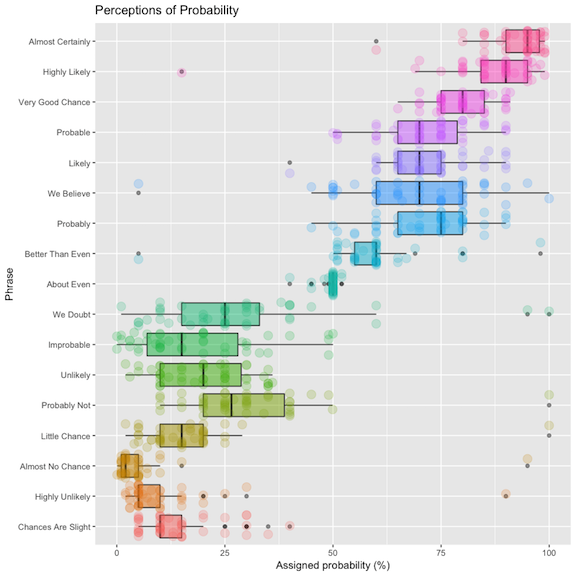
\includegraphics[width=.9\linewidth]{figures/probPlot.png}

As you can see, there is a lot of variability in our perceptions of uncertainty.  Thus, it is very important to know \emph{exactly} what we are talking about when dealing with probability.  We will be very specific about these notions this semester.

So, to start -- What exactly is probability?

Definition: a \textbf{probability} is a function $p(x)$ that assigns "outcomes" $x$ to real numbers $p(x)$ so that the following properties hold:

\begin{enumerate}
\item $p(x)\geq 0$ for any $x$
\item For any two mutually exclusive outcomes $x$ and $y$, we have $p(x\text{ or }y)=p(x)+p(y)$
\item $\sum p(x) = 1$, where the sum is taken over all possible outcomes $x$
\end{enumerate}

Example: verify that the following mapping defines a probability:

\begin{center}
\begin{tabular}{lrrrr}
$x$ & 0 & 1 & 2 & 3\\
$p(x)$ & 0.125 & 0.375 & 0.375 & 0.125\\
\end{tabular}
\end{center}

Note that we can also construct a bar plot of this probability:

\begin{verbatim}
x <- c(0, 1, 2, 3)
p <- c(0.125, 0.375, 0.375, 0.125)
barplot(p, names.arg=x, xlab="x", ylab="p(x)")
\end{verbatim}

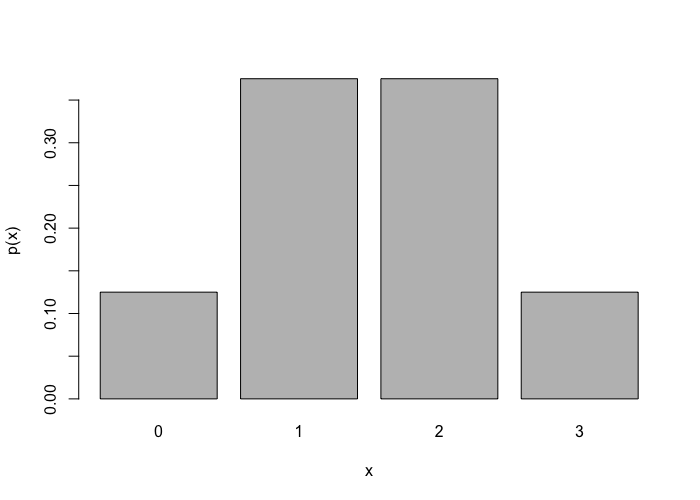
\includegraphics[width=.9\linewidth]{figures/week1/barplot.png}


This bar plot forms an important visualization tool for us called a \textbf{probability distribution}.  We'll talk more about this a bit later.

\subsection*{expected value and variance}
\label{sec-2-2}
Expected value is a generalization of the concept of mean (which you are already quite familiar with).

Definition: the \textbf{expected value} of a random variable $X$ is given by

\[
E(X) = \sum_{x\in X}xp(x)
\]

Expected value is found by multiplying each outcome by its associated probability, and then adding together all resulting products.

Example: consider the example we just did above.  Then

\[
E(X) = \sum_{x\in X}xp(x) = 0\cdot 0.125 + 1\cdot 0.375 +2\cdot 0.375 + 3\cdot 0.125 = 1.5
\]

Note: you can also get the same thing in R very quickly via the following command:

\begin{verbatim}
sum(x*p)
\end{verbatim}

Expected value is a useful concept in many ways:
\begin{itemize}
\item it allows us to define a notion of "mean" for ANY set of outcomes (even an infinite set)
\item it gives us a very quick definition of variance!
\end{itemize}

Example: the \textbf{variance} of a random variable $X$ is defined as $E[(x-\mu)^2]$.

Before we compute this for our example distribution, lets check that it makes sense.  $E[(x-\mu)^2]$ represents our "expectation" of the squared difference from the mean.  That is exactly how variance was defined in your past statistics courses.

Example: consider again our example distribution from earlier.

\begin{center}
\begin{tabular}{lrrrr}
$x$ & 0 & 1 & 2 & 3\\
$p(x)$ & 0.125 & 0.375 & 0.375 & 0.125\\
$x-\mu$ & -1.5 & 0.5 & 0.5 & 1.5\\
$(x-\mu)^2$ & 2.25 & 0.25 & 0.25 & 2.25\\
$(x-\mu)^2\cdot p(x)$ & 0.28125 & 0.09375 & 0.09375 & 0.28125\\
\end{tabular}
\end{center}

So the variance is $E[(x-\mu)^2]$ = 0.28125+0.09375+0.98375+0.28125 = 0.75

As before, this is pretty easy to do in R:

\begin{verbatim}
mu = sum(x*p)
sum((x-mu)^2*p)
\end{verbatim}

\section*{Special Distributions}
\label{sec-3}

Many common probability distributions are given by explicit formulas for their probability functions.  Two that we'll talk about this week are the \textbf{binomial} and \textbf{normal} distributions.

\subsection*{Binomial distribution}
\label{sec-3-1}

The binomial distribution goes back to Bernoulli in 1713.  It arises in situations where each experimental trial has only two outcomes, which we'll call success and failure (such trials are called Bernoulli trials).  

Before presenting the general form of the binomial, lets try a simple example.

Suppose we flipped a fair coin three times.  The probability of landing heads (which we'll call a "success") is $p=0.5$.  Consequently, the probability of landing tails (which we'll call "failure") is $1-p=0.5$.

Let $X$ denote the random variable that counts the number of successes in these three trials.

Some questions:
\begin{enumerate}
\item what are the possible values (outcomes) for $X$?
\item what is the probability of each outcome?
\end{enumerate}

It is easy to see that we get the same probability distribution that we were working with earlier:

\begin{center}
\begin{tabular}{lrrrr}
$x$ & 0 & 1 & 2 & 3\\
$p(x)$ & 0.125 & 0.375 & 0.375 & 0.125\\
\end{tabular}
\end{center}

If we think about this, it is not too difficult to come up with a mathematical process that generates these probabilities for the general case.

Suppose we have $N$ trials, and the probability of success on any one trials is $p$.

Then we know the following:
\begin{enumerate}
\item the probability of each success is $p$
\item the probability of each failure is $1-p$
\item we have $x$ successes
\item we have $N-x$ failures
\item there are ${N\choose x}=\frac{N!}{x!(N-x)!}$ ways to arrange these $x$ successes from the $N$ trials
\end{enumerate}

Thus, the general formula for the binomial probability function is:

\[
p(x) = {N\choose x} p^x(1-p)^{N-x}
\]

\subsubsection*{Example 1}
\label{sec-3-1-1}
A coin is tossed 10 times.  What is the probability of getting exactly 7 heads?

This problem corresponds to a binomial experiment, where there are 10 independent Bernoulli trials, and $p=0.5$.  Then we can calculate the probability via the binomial distribution:

\[
p(x=7) = {10\choose 7} (0.5)^7(0.5)^3
\]

Using R, we can calculate this as:

\begin{verbatim}
choose(10,7)*0.5^7*0.5^3
\end{verbatim}

As we can see from the answer (0.117), this outcome is fairly unlikely

\subsubsection*{Example 2}
\label{sec-3-1-2}
Suppose you run a series of 5 independent replications of an experiment, each with fairly high power (say 80\%).  Suppose there is a true effect; that is, the null hypothesis is false.  What is the probability of getting a significant result (i.e., rejecting the null) in all 5 experiments?

This situation can also be thought of using a binomial distribution.  Each experiment is an independent trial with two outcomes: reject null, or fail to reject null.  The probability of rejecting the null is 0.8.  Then by the binomial distribution, we have

\[
p(x=5) = {5\choose 5} (0.8)^5(0.2)^0 = 0.328
\]

This might be surprising!



\subsubsection*{Some R functions}
\label{sec-3-1-3}

While we can do binomial calcuations from scratch, R has some nice built-in functions to handle these calculations.  Any of the above calculations can be done using the \texttt{dbinom} function.  As an illustration, the two previous examples could be computed using the following commands:

\begin{verbatim}
dbinom(x=7, size=10, prob=0.5)
dbinom(x=5, size=5, prob=0.8)
\end{verbatim}

\subsubsection*{digging deeper -- Likelihoods}
\label{sec-3-1-4}
If we have time, we can talk about an extension of the binomial distribution.  Suppose we flip a coin 10 times, and we see 8 heads.  Do we believe this coin is fair?

Notice that this is a different problem than before.  Here, we are given the number of successes, but NOT the probability of success on any one trial.  This is called a \textbf{likelihood} function.  Let's plot it:

\begin{verbatim}
x = seq(from=0, to=1, by=0.01)
y = dbinom(x=8, size=10, prob=x)
plot(x, y, type="l", xlab="p", ylab="likelihood")
\end{verbatim}

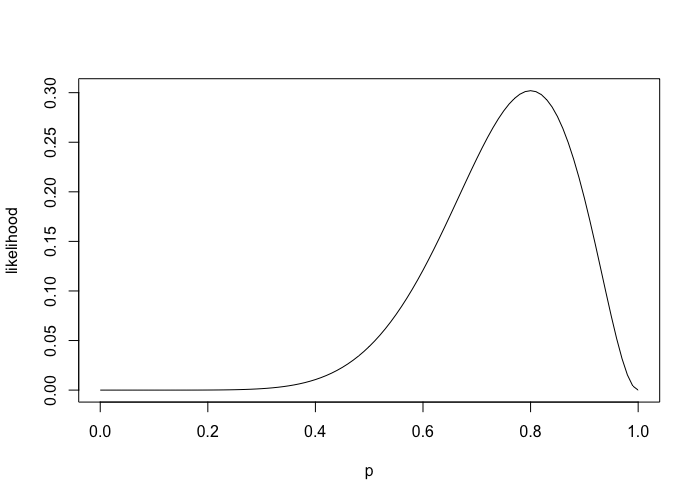
\includegraphics[width=.9\linewidth]{figures/week1/likelihood.png}

This curve tells us which values of $p$ are most likely to give us the data we observed; namely, 8 successes.  Which value of $p$ do you think is \emph{most likely}?

You can test your prediction by adding the command \texttt{abline(v=est)}, where \texttt{est} is the number for $p$ you estimated.

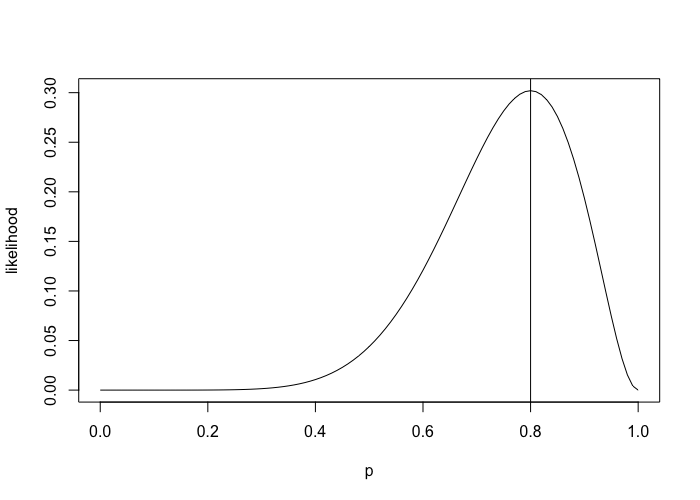
\includegraphics[width=.9\linewidth]{figures/week1/mle.png}

Note: this estimator (0.8 in this case) is called the \textbf{maximum likelihood estimate}.  It is literally the estimate for $p$ which maximizes the likelihood function.  That means it is the estimate for $p$ that is most likely, given the observed data.  This is a fundamental tool in statistical modeling.


\subsection*{Normal distribution}
\label{sec-3-2}
% Emacs 25.2.1 (Org mode 8.2.10)
\end{document}